\documentclass[11pt]{article}
\usepackage{enumerate}
\usepackage{tikz,tikz-cd,tikz-3dplot,pgfplots}
\usepackage{amsmath,amsthm,amssymb,amsfonts,amsthm}
\usepackage{mathrsfs}
\usepackage{bm,bbm}
\usepackage{braket}
\usepackage{slashed}
\usepackage{tensor}
\usepackage{indentfirst}
\usepackage[font=small,labelfont=bf]{caption, subcaption}
\usepackage[a4paper, total={6.5in, 9in}]{geometry}
\usetikzlibrary{decorations.markings,positioning,decorations.pathmorphing}
\allowdisplaybreaks
\pgfplotsset{width=10cm, compat=1.16}
\renewcommand\bra[1]{{\langle{#1}|}}
\renewcommand\ket[1]{{|{#1}\rangle}}
\renewcommand\bfdefault{b}

\newtheorem{theorem}{Theorem}[section]
\newtheorem{lemma}[theorem]{Lemma}
\newtheorem{corollary}{Corollary}[theorem]
\theoremstyle{definition}
\newtheorem{definition}{Definition}[section]
\theoremstyle{remark}
\newtheorem{remark}{Remark}[section]

\DeclareMathOperator{\sech}{sech}
\DeclareMathOperator{\csch}{csch}
\DeclareMathOperator{\arcsec}{arcsec}
\DeclareMathOperator{\arccot}{arccot}
\DeclareMathOperator{\arccsc}{arccsc}
\DeclareMathOperator{\arccosh}{arccosh}
\DeclareMathOperator{\arcsinh}{arcsinh}
\DeclareMathOperator{\arctanh}{arctanh}
\DeclareMathOperator{\arcsech}{arcsech}
\DeclareMathOperator{\arccsch}{arccsch}
\DeclareMathOperator{\arccoth}{arccoth} 

\begin{document}
	\title{In-resonance decay channel detection}
	\author{Seokhyeon Song}
	\maketitle
	
	(Introduction here?)
	
	The exact propagator of a scalar field can be written in a form of
	\[\Delta(p^{2})=\frac{i}{p^{2}-M_{0}^{2}+\Pi(p^{2})},\]
	where the self-energy $\Pi(p^{2})$ contains the sum of 1PI loop integrals.
	Following the ``real on-shell'' renormalisation convention, the propagator is
	\[\Delta(p^{2})=\frac{i}{p^{2}-M^{2}+\Pi(p^{2})-\mathrm{Re}\,\Pi(M^{2})}=\frac{iZ}{p^{2}-M^{2}+iZ\,\mathrm{Im}\,\Pi(p^{2})+O((p^{2}-M^{2})^{2})},\]
	where the real on-shell mass $M$ and the field-strength renormalisation $Z$ satisfy
	\begin{align*}
		M^{2}&=M_{0}^{2}-\mathrm{Re}\,\Pi(M^{2}),\\
		Z^{-1}&=1+\mathrm{Re}\bigg[\frac{d\Pi(p^{2})}{d(p^{2})}\bigg]_{p^{2}=M^{2}}.
	\end{align*}
	(Particles near threshold ref. here)
	The imaginary part of the denominator of the propagator is related to the particle's total decay width $\Gamma$, where
	\[M\Gamma=Z\,\mathrm{Im}\,\Pi(M^{2}).\]
	Because of unitarity, this definition of decay width coincides with the definition given by the scattering amplitude with one initial state. (More rigorous statement needed. Actually only well-defined in NWA?)
	
	One of the alternative definition uses the complex pole mass $\tilde{M}_{p}$, where the propagator diverges at $p^{2}=\tilde{M}_{p}^{2}$.
	In this framework, the real particle mass $M_{p}$ and the width $\Gamma_{p}$ can be read,
	\[\tilde{M}_{p}=M_{p}-\frac{i}{2}\Gamma_{p}.\]
	This definition seems to be mathematically more concise, but there are subtleties.
	In terms of complex plane of $p^{2}$, the physical Riemann sheet consists of the positive-imaginary half plane and its Schwarz reflection.
	In this sheet, the propagator has no pole.
	In order to get a pole, we have to perform analytic continuation across a branch cut starting from $p^{2}=M_{\mathrm{th}}^{2}$, where the ``threshold invariant mass" $M_{\mathrm{th}}$ is a sum of the masses of decay products.
	If there are more than one available decay channels, then there can be more than one secondary Riemann sheets, each contains complex pole.
	
	If all the threshold invariant masses are sufficiently out off the resonance peak, we can analytically continue the Riemann sheet through the branch near the peak and obtain the complex pole, which agrees well with the real on-shell mass and width.
	The reason is that because the self energy $\Pi(p^{2})$ is an analytic function of $p^{2}$ except on the poles and branch singularities, we may linearly approximate
	\[p^{2}-M_{0}^{2}+\Pi(p^{2})\simeq Z_{p}^{-1}(p^{2}-\tilde{M}_{p}^{2})\]
	near the peak, where $Z_{p}^{-1}$ is the residue of propagator on the pole $p^{2}=\tilde{M}_{p}^{2}$.
	Then
	\[\Delta(p^{2})\simeq\frac{iZ_{p}}{p^{2}-\tilde{M}_{p}^{2}}=\frac{iZ_{p}}{p^{2}-(M_{p}^{2}-\frac{\Gamma_{p}^{2}}{4})+iM_{p}\Gamma_{p}},\]
	suggesting Breit-Wigner distribution.
	Typically, decay width of a particle is way smaller than a mass, so we can neglect the $\Gamma_{p}^{2}$ term.
	
	However, if there is an ``in-resonance" decay channel whose threshold invariant mass lies inside the peak, then there exists a branch singularity inside the peak on the real axis, hence such linear approximation is invalid.
	In this case, depending on the point of view, one can say that more than one pole is involving in the resonance, or that no pole explains the resonance well enough.
	Even in this case, the real on-shell definition serves as a definition of the unique mass and width, therefore, the mass and width from now on will only mean the real on-shell values.
	
	\begin{figure}
		\centering
		\begin{subfigure}[b]{0.4\textwidth}
			\centering
			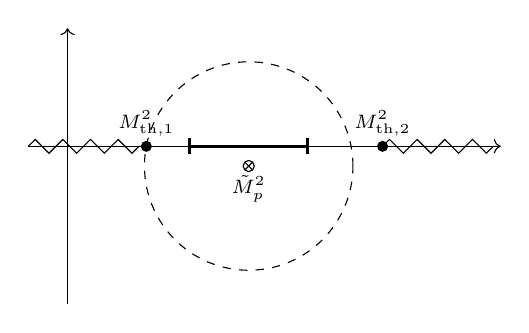
\begin{tikzpicture}
				\draw[->] (-0.5,0) -- (5.5,0);
				\draw[->] (0,-2) -- (0,1.5);
				\draw[decorate,decoration=zigzag] (-0.5,0) -- (1,0);
				\draw[decorate,decoration=zigzag] (4,0) -- (5.5,0);
				\fill (1,0) circle[radius=2pt];
				\fill (4,0) circle[radius=2pt];
				\draw[dashed] (2.3,-0.25) circle[radius=sqrt(1.7525)];
				\draw[very thick] (1.55,0) -- (3.05,0);
				\draw[very thick] (1.55,0.1) -- (1.55,-0.1);
				\draw[very thick] (3.05,0.1) -- (3.05,-0.1);
				\draw (2.25,-0.2) -- (2.35,-0.3);
				\draw (2.25,-0.3) -- (2.35,-0.2);
				\draw (2.3, -0.25) circle[radius=sqrt(2)*0.05];
				\node at (2.3,-0.25) [below]{$\scriptstyle\tilde{M}_{p}^{2}$};
				\node at (1,0) [above]{$\scriptstyle M_{\mathrm{th},1}^{2}$};
				\node at (4,0) [above]{$\scriptstyle M_{\mathrm{th},2}^{2}$};
			\end{tikzpicture}
			\caption{}
			\label{fig:pole_structure:out_peak}
		\end{subfigure}
		\begin{subfigure}[b]{0.3\textwidth}
			\centering
			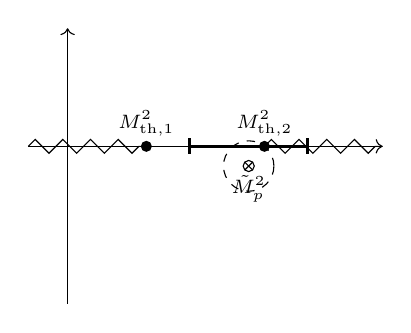
\begin{tikzpicture}
				\draw[->] (-0.5,0) -- (4,0);
				\draw[->] (0,-2) -- (0,1.5);
				\draw[decorate,decoration=zigzag] (-0.5,0) -- (1,0);
				\draw[decorate,decoration=zigzag] (2.5,0) -- (4,0);
				\fill (1,0) circle[radius=2pt];
				\fill (2.5,0) circle[radius=2pt];
				\draw[dashed] (2.3,-0.25) circle[radius=sqrt(0.1025)];
				\draw[very thick] (1.55,0) -- (3.05,0);
				\draw[very thick] (1.55,0.1) -- (1.55,-0.1);
				\draw[very thick] (3.05,0.1) -- (3.05,-0.1);
				\draw (2.25,-0.2) -- (2.35,-0.3);
				\draw (2.25,-0.3) -- (2.35,-0.2);
				\draw (2.3, -0.25) circle[radius=sqrt(2)*0.05];
				\node at (2.3,-0.25) [below]{$\scriptstyle\tilde{M}_{p}^{2}$};
				\node at (1,0) [above]{$\scriptstyle M_{\mathrm{th},1}^{2}$};
				\node at (2.5,0) [above]{$\scriptstyle M_{\mathrm{th},2}^{2}$};
			\end{tikzpicture}
			\caption{}
			\label{fig:pole_structure:in_peak}
		\end{subfigure}
		\captionsetup{width=.9\linewidth}
		\caption{Diagrams demonstrating complex-analytic structure of the propagator $\Delta(p^{2})$, drawn on a complex plane of $p^{2}$. The thick interval indicates the range of resonance peak, and the Riemann sheet is analytically continued through the midpoint of peak. The small circles with cross displays the position of a pole on a secondary Riemann sheet, and the dashed circles means the radius of convergence of the self-energy function $\Pi(p^{2})$, centered on the pole. (a) If every threshold invariant masses are far from the peak, the entirety of peak lies well inside the radius of convergence. Hence, we can take a linear approximation of the self-energy. (b) If there is a threshold invariant mass inside the peak, the self-energy is non-analytic. Thus a linear approximation breaks down.}
		\label{fig:pole_structure}
	\end{figure}
	
	\section{}
	In the presence of in-resonance decay channel, a shape of resonance peak does not resemble the Breit-Wigner distribution, and a nontrivial momentum dependence of a self-energy becomes important.
	
	In one-loop correction of the scalar propagator, such momentum dependence is most pronounced when the loop particles are scalars.
	In this case, the propagator is non-differentiable at the threshold, resulting in a characteristic kink shape.
	For higher-spin loop particles, the difference from the Breit-Wigner distribution is small even when the coupling constant is large.
	Looking only at the imaginary component, higher-spin decay products suffers large phase space suppression because the mother particle mass is very close to the threshold.
	Thus, particles with spin do not contribute significantly to the decay width, suggesting a minor effect on the overall resonance shape.
	
	이 윗부분을 그냥 제대로 Lagrangian 도입해서 다시 쓰는 게 좋을 듯. 결과도 그래프로 보여주고.
	
	(I have to write something here, but I can't think of anything right now)
	
	If a background scattering amplitude is nearly constant within the range of resonance peak, the maximum likelihood fitting can be approximated by least squares fitting.
	Then the $\chi^{2}$ test statistic is proportional to the total squared residue times total luminosity.
	
\end{document}